\section{Metodologia}

\subsection{Distribuição Normal com Tabuleiro de Galton}

Foi utilizado um tabuleiro de Galton para ilustrar a distribuição normal. Bolinhas foram lançadas de forma controlada, passando por diversos pinos distribuídos simetricamente, o que provocou trajetórias aleatórias e resultou na formação de uma curva em forma aproximada de sino ao final do experimento. Durante a atividade, tomou-se o cuidado de inserir as bolinhas lentamente para evitar sua queda fora do sistema. A \cref{fig:galton} mostra o aparato experimental utilizado.

\begin{figure}[H]
\centering
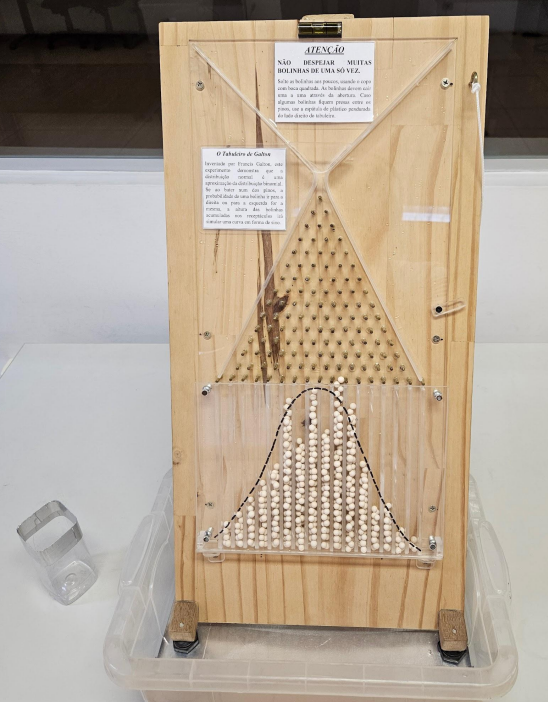
\includegraphics[width=0.35\linewidth]{fig/galton.png}
\caption{Tabuleiro de Galton utilizado para simular uma distribuição normal. As bolinhas atravessam um arranjo simétrico de pinos, distribuindo-se em compartimentos inferiores. Fonte: fotografia tirada pelo monitor da disciplina.}
\label{fig:galton}
\end{figure}

\subsection{Distribuição Normal e Estouro de Pipocas}

O comportamento estatístico do estouro de pipocas foi usado como analogia para a distribuição normal. Pipocas foram aquecidas em um forno De micro-ondas, e a sequência de estouros foi registrada por um gravador de celular. 

\subsection{Pressão do Ar e Gás Ideal em Garrafa}

Utilizou-se uma garrafa plástica parcialmente preenchida com ar para estimar a pressão interna do gás. Com o auxílio de uma bomba manual acoplada a uma tampa adaptada, foi possível injetar diferentes quantidades de ar, garantindo a vedação do sistema. A pressão no interior da garrafa foi então medida com um equipamento apropriado. Para determinar a variação de massa, a garrafa foi pesada antes e depois da injeção de ar utilizando uma balança de precisão. A \cref{fig:garrafa} mostra a montagem experimental.

\begin{figure}[H]
\centering
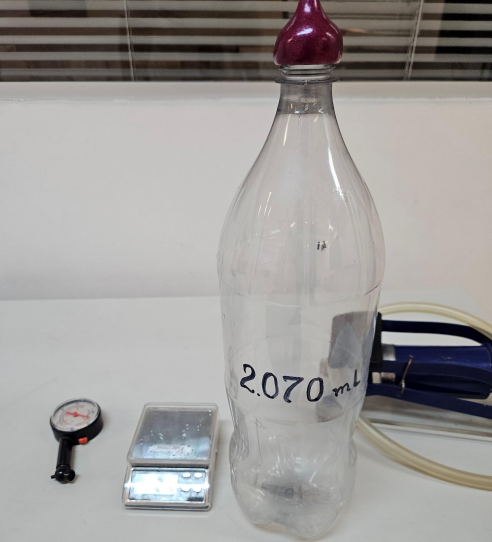
\includegraphics[width=0.40\linewidth]{fig/garrafa.png}
\caption{Garrafa com sistema vedado para injeção de ar por bomba manual. A pressão foi medida após cada etapa, e a massa, comparada por pesagem. Fonte: imagem capturada pelo monitor Pedro.}
\label{fig:garrafa}
\end{figure}

\subsection{Motor de Teoria Cinética dos Gases}

O experimento utilizou um motor demonstrativo da teoria cinética dos gases. Nele, bolinhas plásticas representando moléculas colidiam aleatoriamente com as paredes internas de um cilindro e com um êmbolo móvel foram agitadas por um motor elétrico conectado à base do equipamento. O movimento das bolinhas provocava o deslocamento do êmbolo. Por precaução, o sistema não foi mantido ligado por longos períodos, conforme orientação. A \cref{fig:cinetica} mostra o aparato experimental.

\begin{figure}[H]
\centering
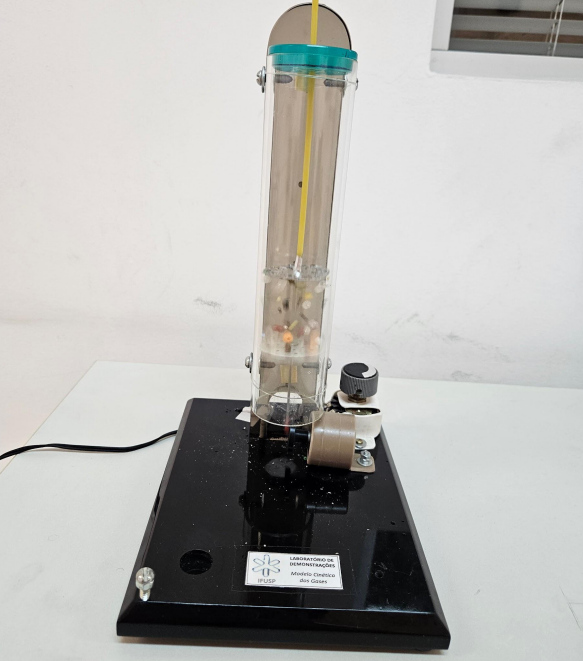
\includegraphics[width=0.45\linewidth]{fig/cinetica.png}
\caption{Equipamento representando a teoria cinética dos gases. As bolinhas são agitadas por um motor na base, simulando colisões com o êmbolo móvel. Fonte: fotografia obtida pelo monitor da disciplina.}
\label{fig:cinetica}
\end{figure}
